\documentclass[compress]{beamer}
\usetheme{sthlm}

%-=-=-=-=-=-=-=-=-=-=-=-=-=-=-=-=-=-=-=-=-=-=-=-=
%        LOADING BEAMER PACKAGES
%-=-=-=-=-=-=-=-=-=-=-=-=-=-=-=-=-=-=-=-=-=-=-=-=

\usepackage{
booktabs,
datetime,
dtk-logos,
graphicx,
multicol,
pgfplots,
ragged2e,
tabularx,
tikz,
wasysym,
multirow,
float,
caption,
subcaption
}

\pgfplotsset{compat=1.8}

\usepackage[utf8]{inputenc}
\usepackage[portuguese]{babel}
\usepackage[T1]{fontenc}
\usepackage{newpxtext,newpxmath}
\usepackage{listings}

\lstset{ %
language=[LaTeX]TeX,
basicstyle=\normalsize\ttfamily,
keywordstyle=,
numbers=left,
numberstyle=\tiny\ttfamily,
stepnumber=1,
showspaces=false,
showstringspaces=false,
showtabs=false,
breaklines=true,
frame=tb,
framerule=0.5pt,
tabsize=4,
framexleftmargin=0.5em,
framexrightmargin=0.5em,
xleftmargin=0.5em,
xrightmargin=0.5em
}



%-=-=-=-=-=-=-=-=-=-=-=-=-=-=-=-=-=-=-=-=-=-=-=-=
%        LOADING TIKZ LIBRARIES
%-=-=-=-=-=-=-=-=-=-=-=-=-=-=-=-=-=-=-=-=-=-=-=-=

\usetikzlibrary{
backgrounds,
mindmap
}

%-=-=-=-=-=-=-=-=-=-=-=-=-=-=-=-=-=-=-=-=-=-=-=-=
%        BEAMER OPTIONS
%-=-=-=-=-=-=-=-=-=-=-=-=-=-=-=-=-=-=-=-=-=-=-=-=

\setbeameroption{show notes}

%-=-=-=-=-=-=-=-=-=-=-=-=-=-=-=-=-=-=-=-=-=-=-=-=
%        BEAMER COMMANDS
%-=-=-=-=-=-=-=-=-=-=-=-=-=-=-=-=-=-=-=-=-=-=-=-=


%-=-=-=-=-=-=-=-=-=-=-=-=-=-=-=-=-=-=-=-=-=-=-=-=
%
%	PRESENTATION INFORMATION
%
%-=-=-=-=-=-=-=-=-=-=-=-=-=-=-=-=-=-=-=-=-=-=-=-=

\title{Introdução a Sistemas \\ Distribuídos}
\subtitle{DCE540 - Computação Paralela e Distribuída}
%\date{\small{\jobname}}
\author{\texttt{Iago Carvalho}}
\institute{\texttt{Departamento de Ciência da Computação}}

\hypersetup{
pdfauthor = {Iago A. Carvalho},      
pdfsubject = {Computação Paralela e Distribuída},
pdfkeywords = {},  
pdfmoddate= {D:\pdfdate},          
pdfcreator = {WriteLaTeX}
}

\begin{document}

\begin{frame}
\titlepage

\end{frame}

%% --------------------------------------------------------

\begin{frame}{Um pouco de história}

A criação dos computadores no pós-guerra mudou o mundo.

\vspace{0.5cm}

Até meados dos anos 1970, os computadores eram
\begin{itemize}
    \item Pesados;
    \item Grandes;
    \item Caros
\end{itemize}

\vspace{0.5cm}

\begin{columns} % align columns
\begin{column}{.48\textwidth}

Devido a estas características e a falta de boas maneiras de conectar um PC a outro, cada máquina operava tradicionalmente isolada das outras.

\end{column}%
\hfill%
\begin{column}{.48\textwidth}


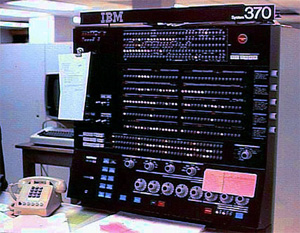
\includegraphics[width=0.85\textwidth]{images/ibm_370.jpg}
\end{column}%
\end{columns}

\end{frame}

%% --------------------------------------------------------

\begin{frame}{Um pouco de história}

A partir de meados de 1980, duas tecnologias mudaram este panorama

\vspace{0.5cm}

\begin{enumerate}
    \item Desenvolvimento de micro-computadores
    \begin{itemize}
        \item Pequenos
        \item Boa capacidade de processamento
        \item Criação de chips multi-core
    \end{itemize}
    \vspace{0.5cm}
    \item Criação das redes locais (LAN)
    \begin{itemize}
        \item Possibilidade de conectar diversos computadores
        \item Troca de grandes quantidades de dados
        \item Comunicação rápida
        \item Internet
        \item Wider-area Networks (WAN)
    \end{itemize}
\end{enumerate}

\end{frame}

%% --------------------------------------------------------

\begin{section}{Um \textbf{sistema distribuído} é uma coleção de elementos de computação autônomos que o usuário enxerga como um sistema único coerente}
\end{section}

%% --------------------------------------------------------

\begin{frame}{Sistemas distribuídos}

Duas principais características de um sistema distribuído

\begin{enumerate}
    \item Coleção de elementos de computação autônomos
    \item Sistema único coerente
\end{enumerate}

\centering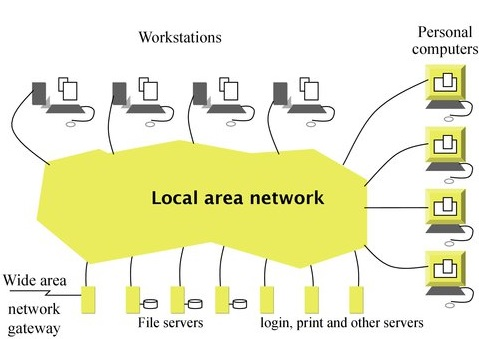
\includegraphics[width=0.8\textwidth]{images/laboratorio.jpg}

\end{frame}

%% --------------------------------------------------------

\begin{frame}{Coleção de elementos de computação autônomos}

Um elemento de computação autônomo é denominado \textbf{nó}
\begin{columns}[T] % align columns
\begin{column}{.40\textwidth}
\begin{itemize}
    \item Celulares
    \item Computadores pessoais
    \item Grandes servidores
    \item Máquinas virtuais
\end{itemize}
\end{column}
\begin{column}{.50\textwidth}
\centering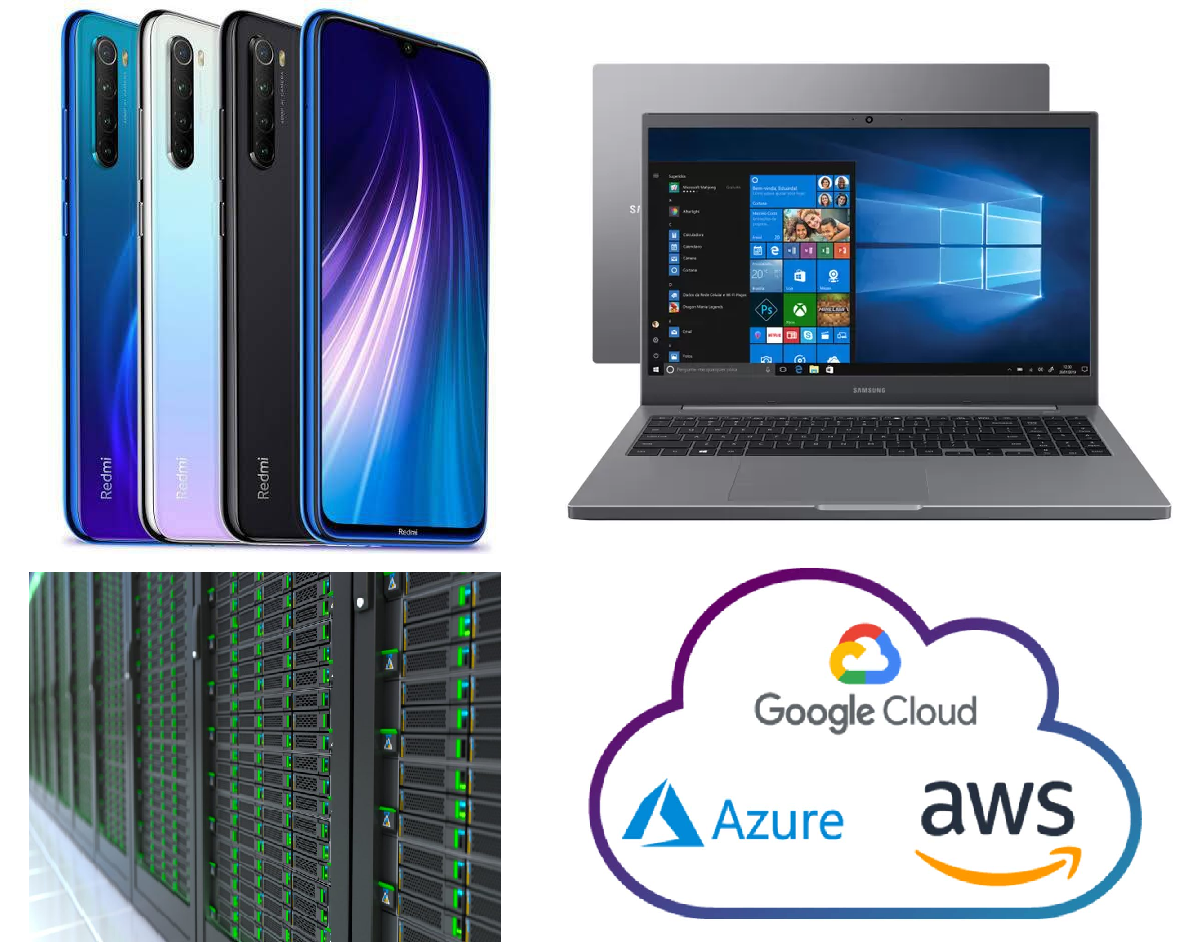
\includegraphics[width=0.8\textwidth]{images/elementos_sd.png}
\end{column}
\end{columns}

\vspace{0.5cm}

Cada nó deve ser capaz de operar de forma independente

\vspace{0.5cm}

Entretanto, não faz sentido um nó ignorar os outros nós de um sistema distribuído

\end{frame}

%% --------------------------------------------------------

\begin{frame}{Coleção de elementos de computação autônomos}

Cada nó deve interagir com os outros nós da rede
\begin{itemize}
    \item Receber mensagens
    \item Enviar mensagens
    \item Processar dados e requisições
\end{itemize}

\vspace{0.5cm}

Os nós devem atuar em conjunto para atingir um objetivo em comum
\begin{itemize}
    \item Gerar uma enorme capacidade de processamento de dados
    \item Disponibilizar recursos para os usuários
    \item Possibilitar a comunicação rápida entre os usuários do sistema
    \item $\ldots$
\end{itemize}
\end{frame}

%% --------------------------------------------------------

\begin{frame}{Coleção de elementos de computação autônomos}

Entretanto, existem algumas dificuldades inerentes ao se montar esta coleção de nós

\vspace{0.5cm}
\begin{itemize}
    \item Sincronização
    \vspace{0.5cm}
    \item Replicação
    \vspace{0.5cm}
    \item Comunicação
    \vspace{0.5cm}
    \item Gerenciamento de dispositivos e ornanização
    \vspace{0.5cm}
    \item Autenticação e segurança
\end{itemize}

\end{frame}

%% --------------------------------------------------------

\begin{frame}{Sistema único coerente}

Idealmente, um usuário deve enxergar, trabalhar e executar um sistema único coerente
\begin{itemize}
    \item Usuário não deve ser capaz de notar que está trabalhando com um sistema distribuído
    \item Não deve saber (ou se preocupar) com onde estão seus dados ou onde seus processos estão rodando
\end{itemize}

\vspace{0.5cm}

Entretanto, obter um sistema único coerente é quase que uma utopia

Assim, espera-se ofertar ao usuário, ao menos, uma visão única coerente
\begin{itemize}
    \item O sistema deve executar de forma similar independente do dispositivo utilizado pelo usuário
\end{itemize}

\end{frame}

%% --------------------------------------------------------

\begin{section}{A distributed system is the "(...) one in which the failure of a computer you didn't even know existed can render your own computer unusable" \\ 
\vspace{1cm}\hspace{5cm} \textbf{Leslie Lamport}}

\end{section}

%% --------------------------------------------------------

\begin{frame}{Middlewares}

Um middleware é um \textit{software} específico que gerencia os recursos de um sistema distribuído
\begin{itemize}
    \item Tarefa semelhante a de um sistema operacional para um computador
\end{itemize}

\vspace{0.5cm}

\centering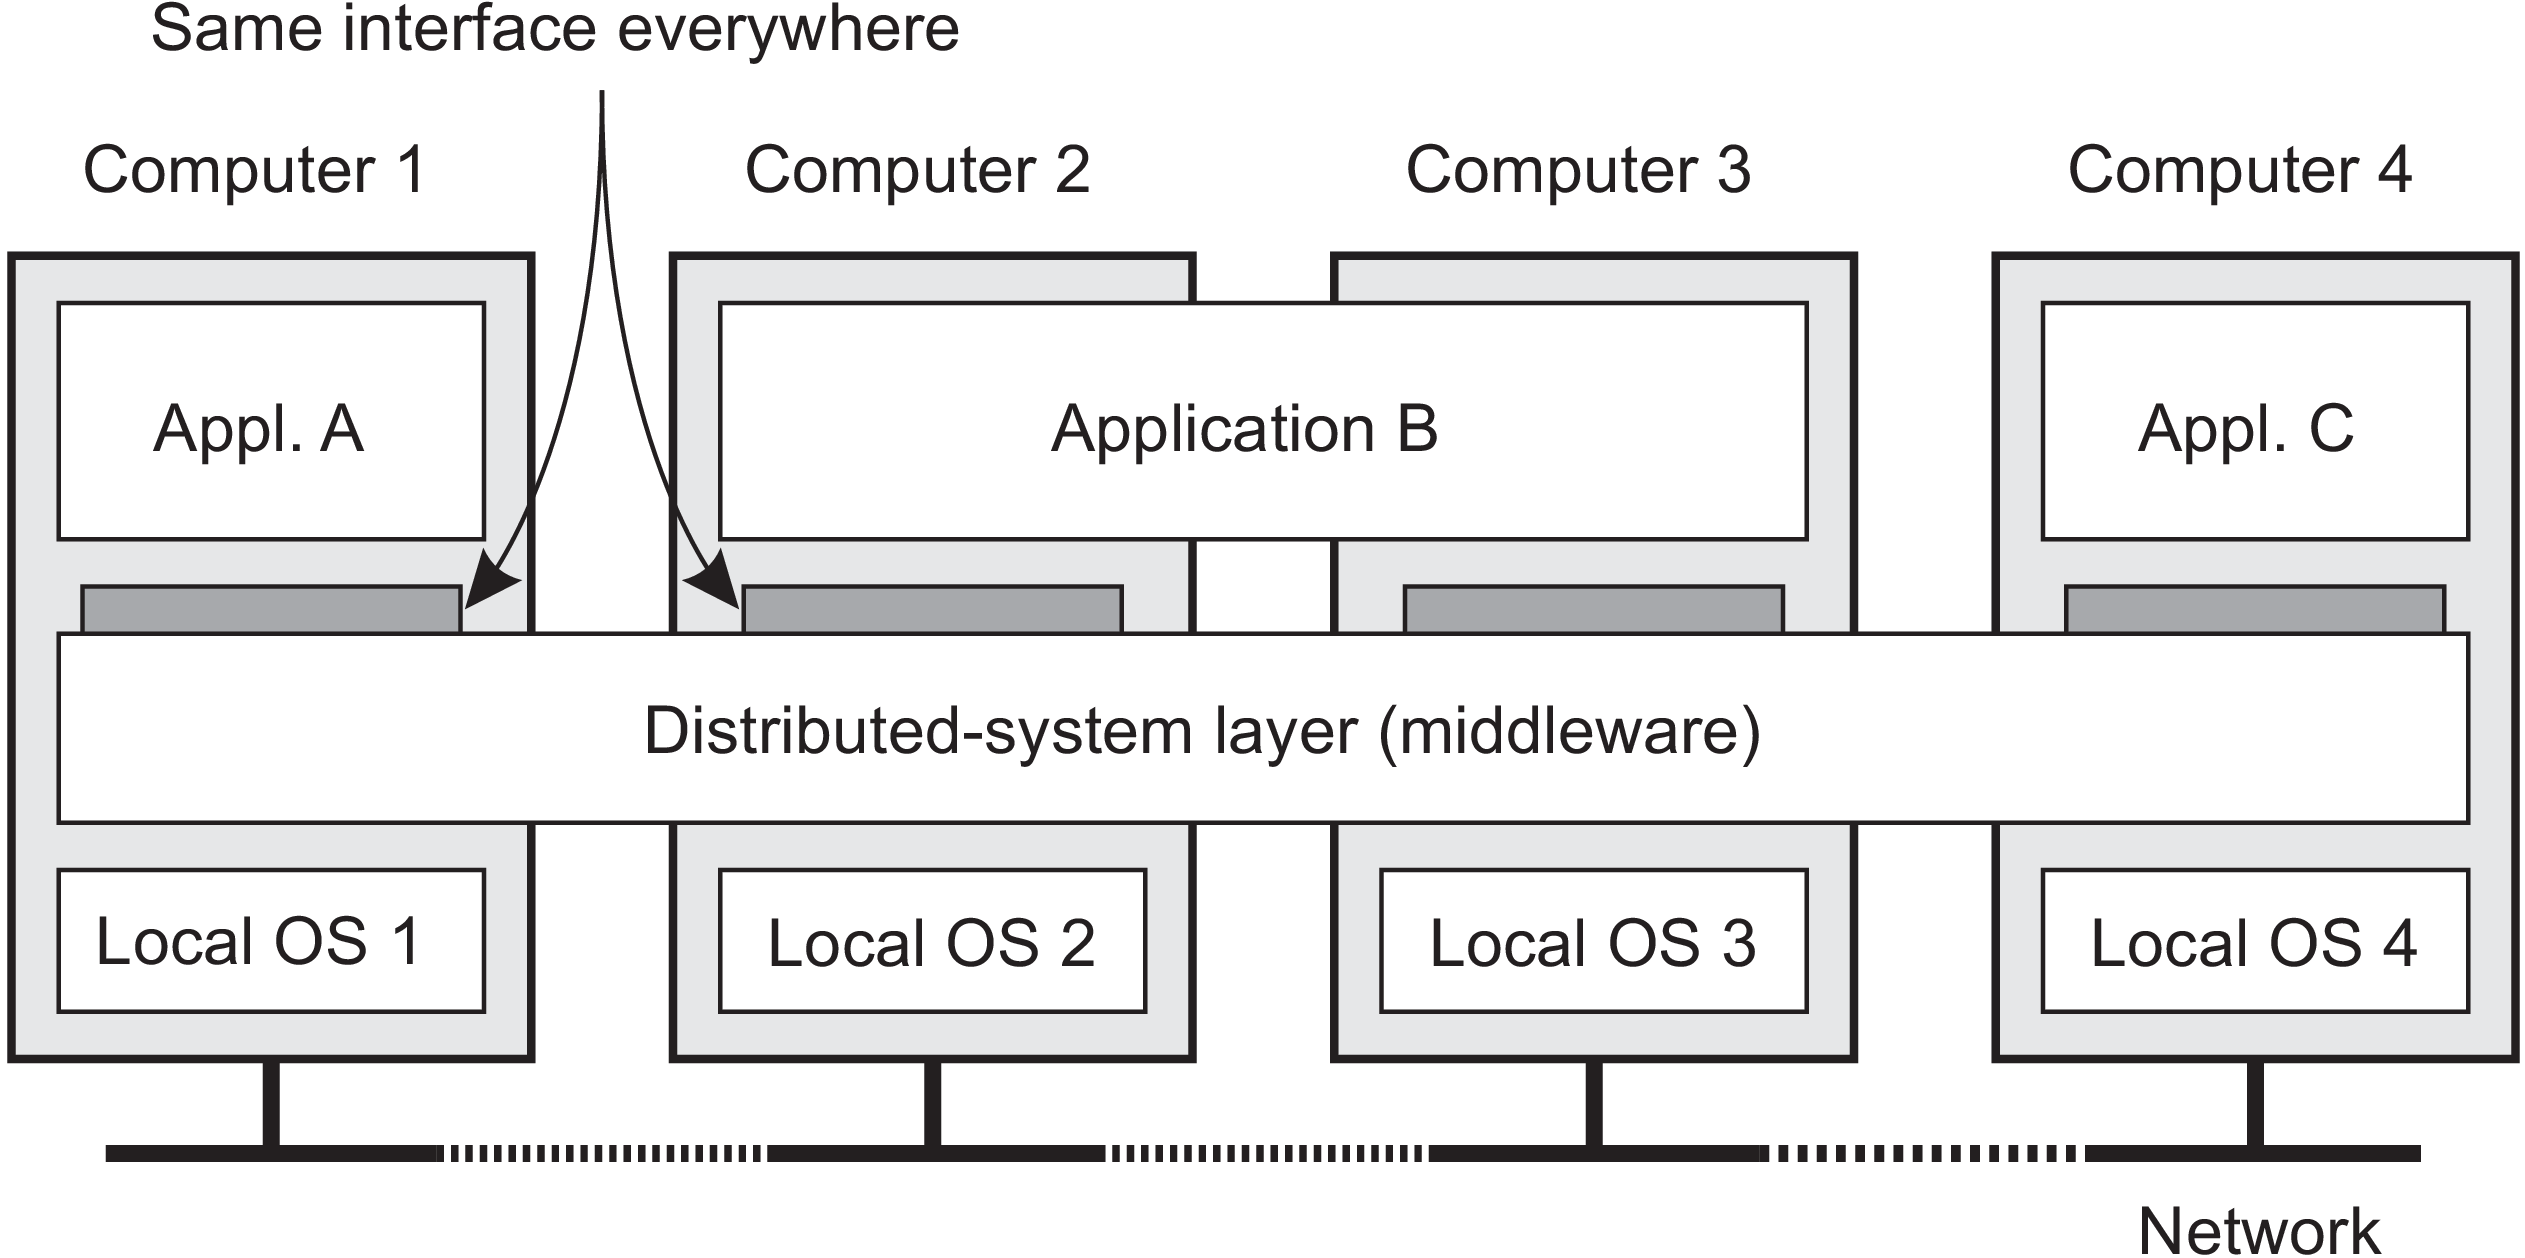
\includegraphics[width=0.9\textwidth]{images/middleware.png}

\end{frame}

%% --------------------------------------------------------

\begin{frame}{Middlewares}

Um middleware deve prover quatro serviços básicos
\begin{enumerate}
    \item Métodos de comunicação
    \item Segurança
    \item Gerenciamento de recursos
    \item Mascaramento e recuperação de falhas
\end{enumerate}

\vspace{0.5cm}

Estes serviços são implementados no middleware e podem ser utilizados por quaisquer aplicações como softwares caixa-preta

\end{frame}

%% --------------------------------------------------------

\begin{frame}{Middlewares - RPC}

Remote Procedure Call (RPC)

\vspace{1cm}

\centering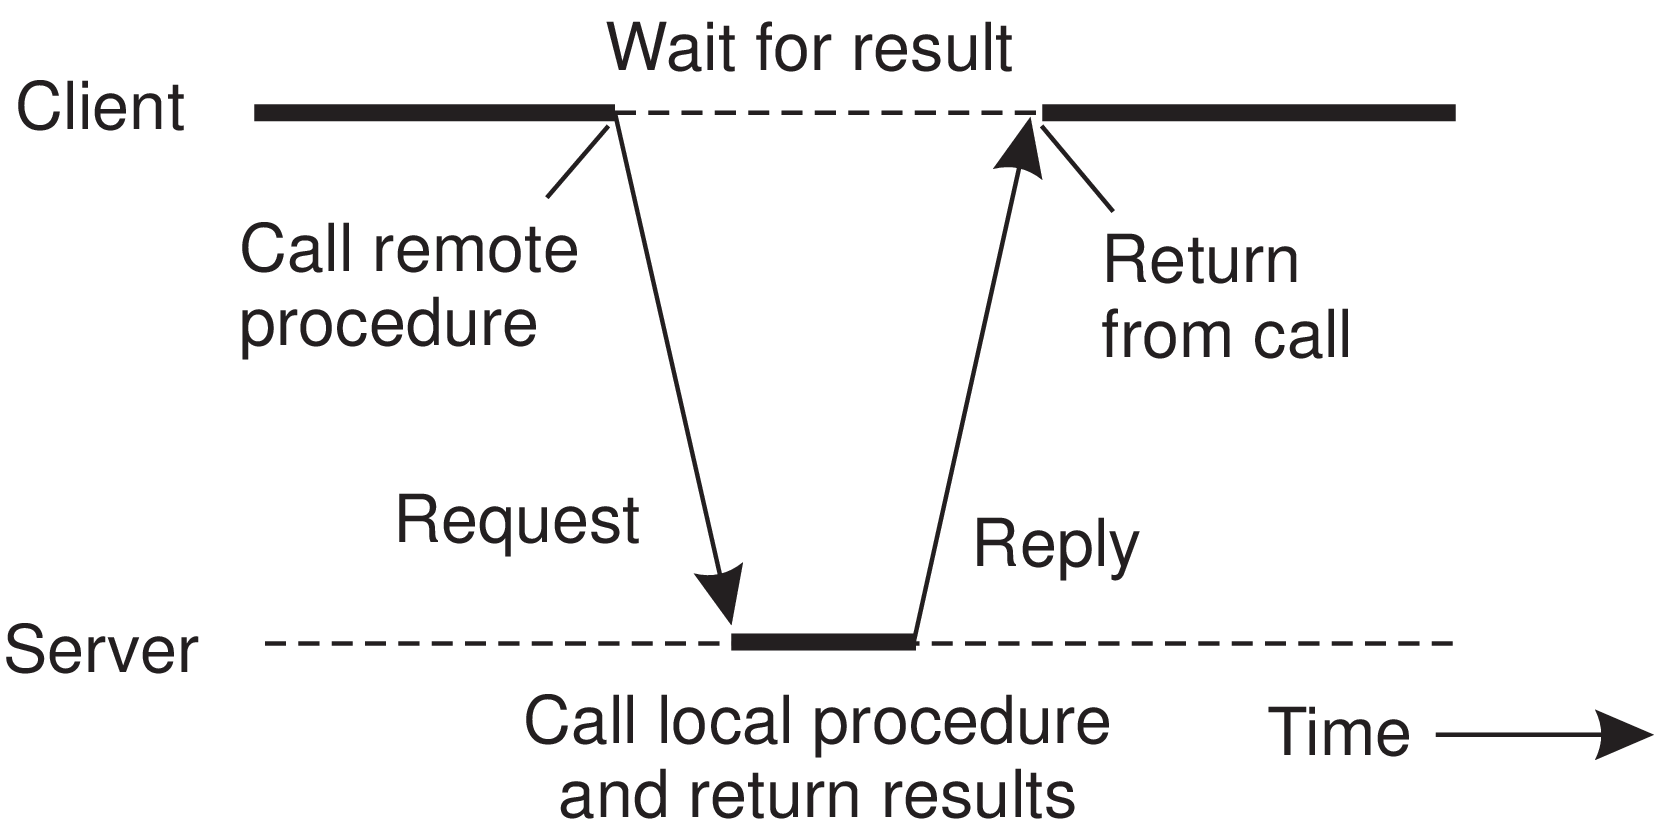
\includegraphics[width=0.9\textwidth]{images/rpc.png}

\end{frame}

%% --------------------------------------------------------

\begin{frame}{Objetivos de um sistema distribuído}

A implementação de um sistema distribuído \textbf{deve} levar em consideração quatro objetivos

\vspace{1cm}

\begin{enumerate}
    \item Recursos devem ser facilmente acessíveis
    \item Localização dos recursos deve ser transparente para o usuário
    \item O sistema tem que ser aberto
    \item O sistema tem que ser escalável
\end{enumerate}

\end{frame}

%% --------------------------------------------------------

\begin{frame}{Acessibilidade de recursos}

Recurso é um termo genérico
\begin{columns}[T]
    \begin{column}{.3\textwidth}
        \begin{itemize}
            \item Periféricos
            \item Dados
            \item Discos rígidos
        \end{itemize}
    \end{column}
    \begin{column}{.48\textwidth}
        \begin{itemize}
            \item Serviços
            \item Redes
            \item Processamento
        \end{itemize}
    \end{column}
\end{columns}

\vspace{1cm}

Recursos facilmente acessíveis proporcionam
\begin{itemize}
    \item Economia \$\$
    \item Facilitam a colaboração e troca de informação
\end{itemize}
\end{frame}

%% --------------------------------------------------------

\begin{frame}{Acessibilidade de recursos}

Redes Peer-2-Peer (P2P)

\vspace{0.5cm}

\centering 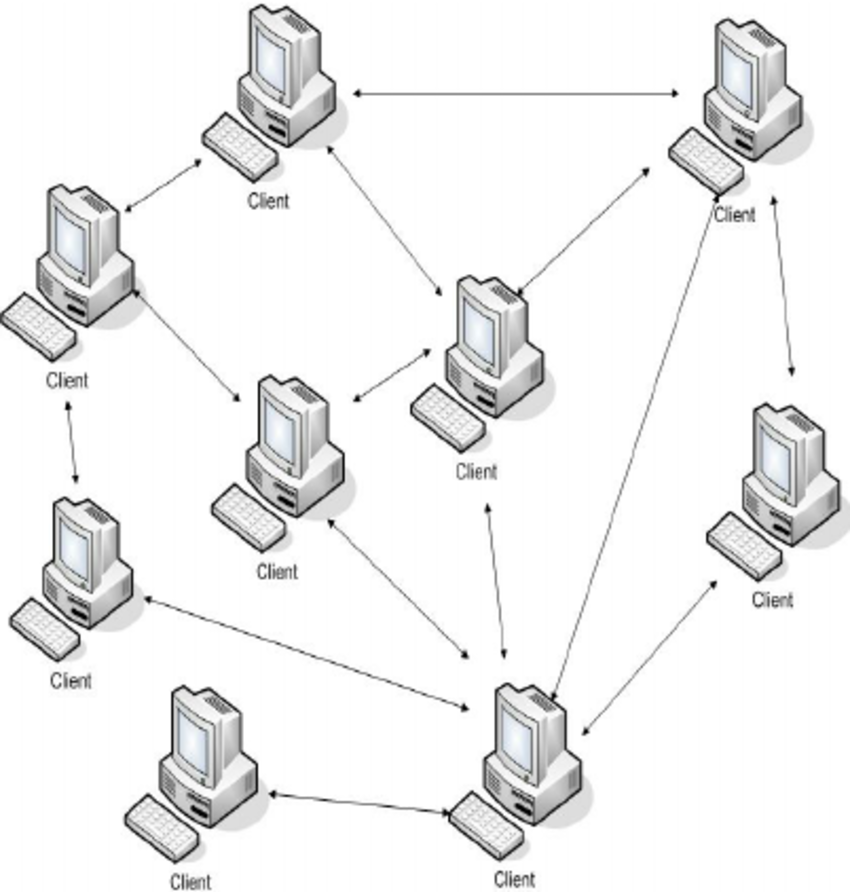
\includegraphics[width=0.6\textwidth]{images/p2p.png}
\end{frame}

%% --------------------------------------------------------

\begin{frame}{Transparência}

Um usuário não deve saber (ou se preocupar) com a localização dos recursos que está utilizando

\begin{table}[]
\centering
\resizebox{\textwidth}{!}{%
\begin{tabular}{@{}ll@{}}
\toprule
\multicolumn{1}{c}{\textbf{Transparência}} & \multicolumn{1}{c}{\textbf{Descrição}}                    \\ \midrule
Acesso      & Forma de representar e acessar os dados \\
Localização & Localização do recurso                  \\
Relocação                                  & Recurso é movido de localização durante o uso             \\
Migração    & Recurso é movido de localização         \\
Replicação  & Recursos replicados                     \\
Concorrência                               & Recursos utilizados simultaneamente por diversos usuários \\
Falha       & Falhas e recuperação de recursos        \\ \bottomrule
\end{tabular}%
}
\end{table}


\end{frame}

%% --------------------------------------------------------

\begin{frame}{Sistema aberto}

Um sistema aberto deve oferecer componentes que podem ser facilmente utilizados por usuários

\vspace{0.5cm}

Além disso, um sistema aberto também deve fornecer meios de integração com outras aplicações ou sistemas
\begin{itemize}
    \item Prover uma interface simples e amigável
    \begin{itemize}
        \item Boa documentação
        \item Implementação bem encapsulada
        \item Baixo acomplamento
    \end{itemize}
\end{itemize}

\end{frame}

%% --------------------------------------------------------

\begin{frame}{Sistema escalável}

Um sistema distribuído deve ser capaz de crescer em três dimensões
\begin{enumerate}
    \item Tamanho
    \begin{itemize}
        \item Facilmente extensível para novos nós e usuários
        \item Sem perca de desempenho
    \end{itemize}
    \item Localização geográfica
    \begin{itemize}
        \item Acesso ao sistema deve ser rápido e eficiente de qualquer lugar
    \end{itemize}
    \item Administrativa
    \begin{itemize}
        \item O crescimento do sistema deve ser facilmente administrável
        \item Políticas universais de uso, administração e segurança
    \end{itemize}
\end{enumerate}

\end{frame}

%% --------------------------------------------------------

\begin{frame}{Tecnicas de escabalibilidade}


\begin{itemize}
    \item Particionamento e distribuição
    \item Replicação de dados
    \begin{itemize}
        \item Cuidados necessários com consistência
    \end{itemize}
    \item Cache de dados
    \begin{itemize}
        \item Cuidados necessários com consistência
    \end{itemize}
    \item Diminuir (ou pelo menos, esconder) latência de acesso
    \begin{itemize}
        \item Comunicação assíncrona
    \end{itemize}
\end{itemize}


\end{frame}

%% --------------------------------------------------------

\begin{frame}{Tipos de sistemas distribuiídos}

Existem três principais tipos de sistemas distribuídos

\begin{itemize}
    \item Sistemas de computação distribuída de alta performance
    \item Sistemas de informação distribuídos
    \item Sistemas pervasivos
\end{itemize}

\end{frame}

%% --------------------------------------------------------

\begin{frame}{Sistemas de computação distribuída de alta performance}

Tem como objetivo processar uma quantidade massiva de dados
\begin{itemize}
    \item Fortemente associado ao conceito de programação paralela
\end{itemize}

\vspace{1cm}

Algumas estruturas são possíveis
\begin{itemize}
    \item Clusters
    \item Grids
    \item Cloud
\end{itemize}
\end{frame}

%% --------------------------------------------------------

\begin{frame}{Cluster}

Uma coleção de nós similares conectados utilizando uma rede de alta velocidade

\vspace{1cm}

\centering 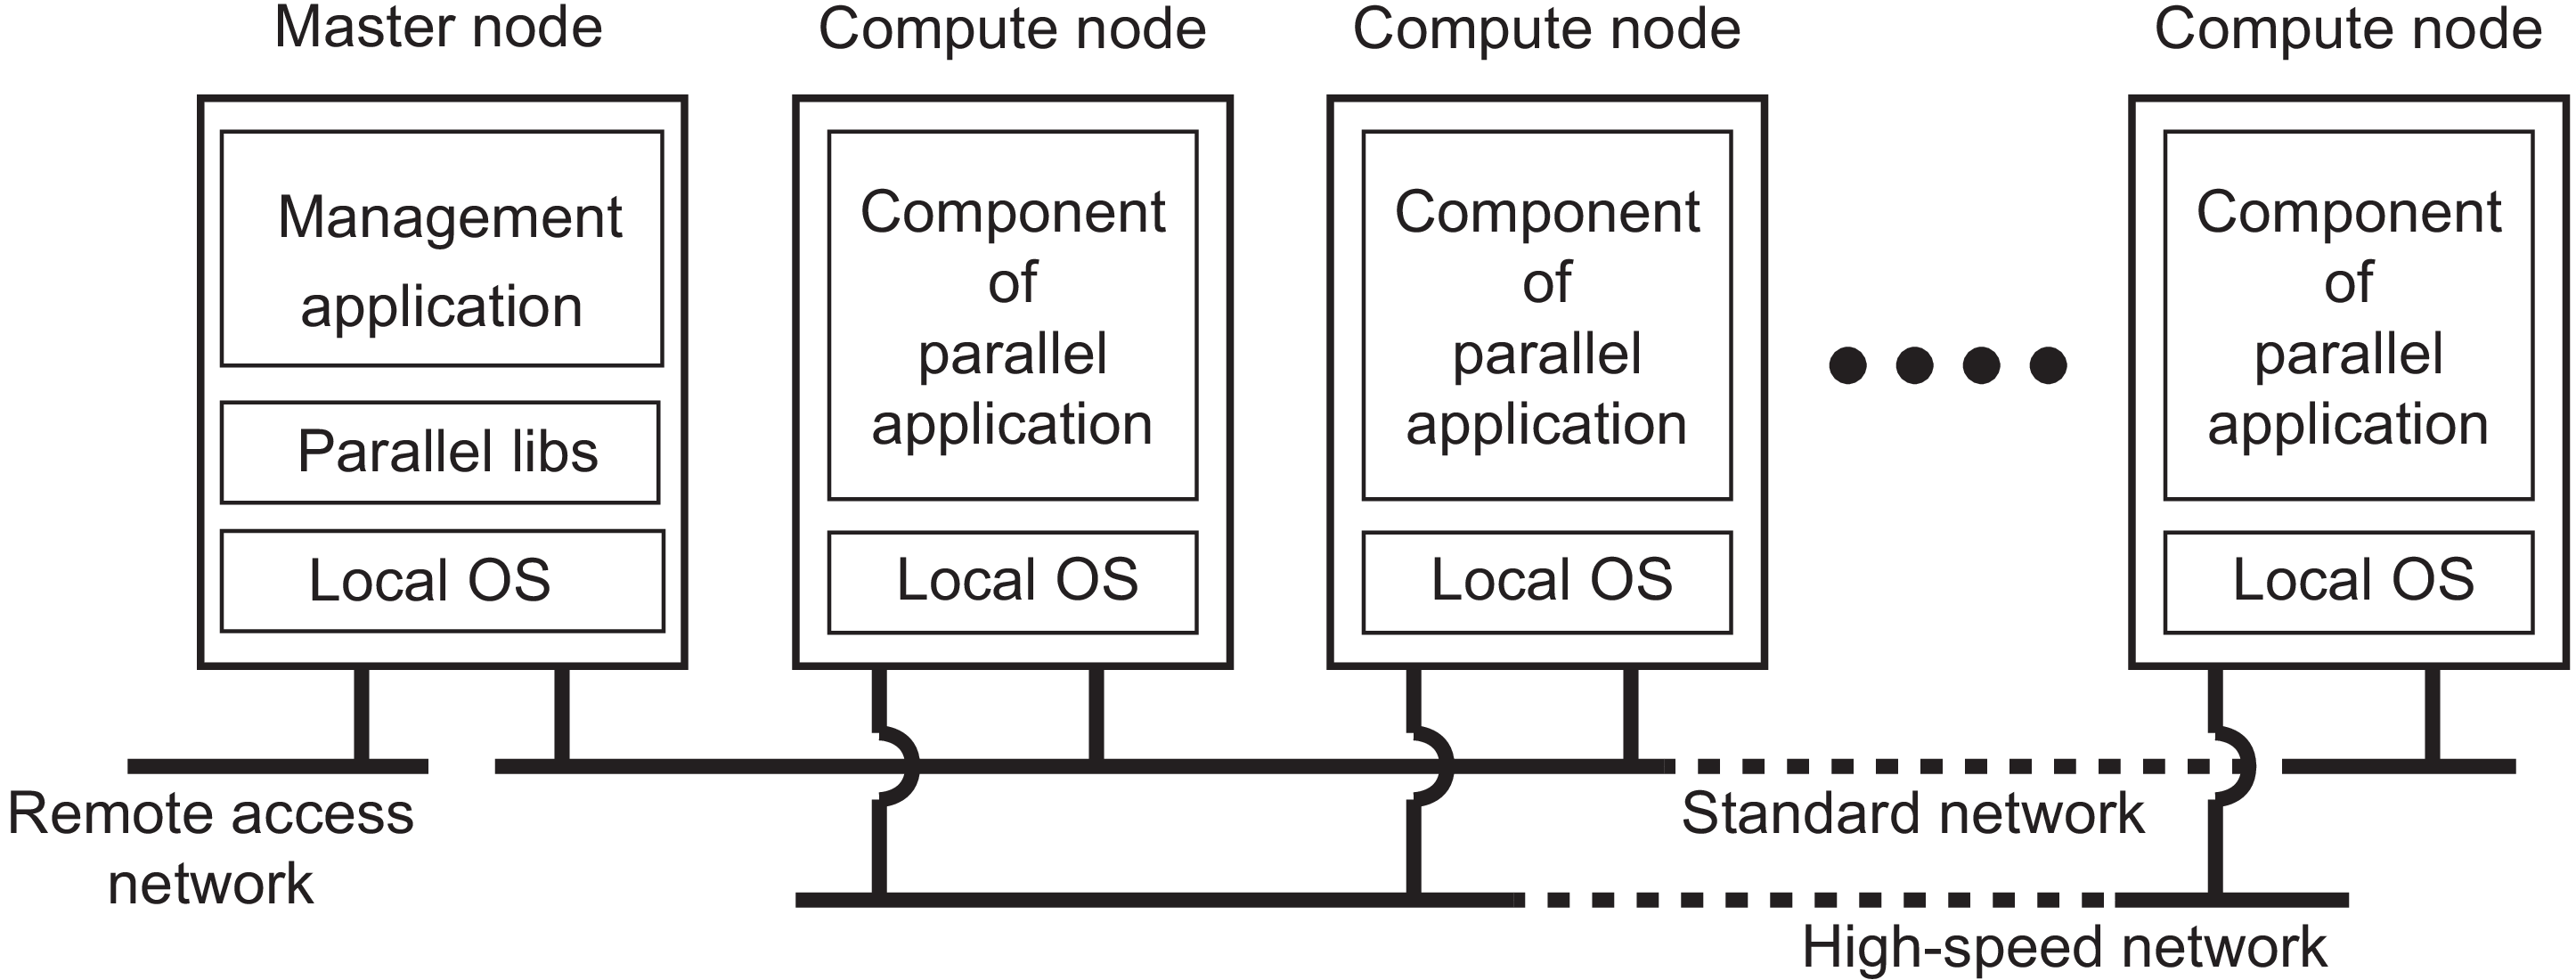
\includegraphics[width=\textwidth]{images/cluster.png}

\end{frame}

%% --------------------------------------------------------

\begin{frame}{Grid}

Muito parecido com um cluster

\vspace{0.5cm}

Entretanto, em um grid, os nós não necessariamente são similares
\begin{itemize}
    \item Diferentes localizações
    \item Diferentes recursos
\end{itemize}

\vspace{0.5cm}

Apesar disso, o acesso e a utilização ainda tem que ser transparente
\end{frame}

%% --------------------------------------------------------

\begin{frame}{Cloud}

\begin{columns}[T]
    \begin{column}{.35\textwidth}
        Objetivo diferente de clusters e grids
        \begin{itemize}
        \item Prover infraestrutura (IaaS)
        \item Diferentes aplicações
        \item Grande número de aplicações    
        \end{itemize}
    \end{column}
    \begin{column}{.72\textwidth}
        \centering 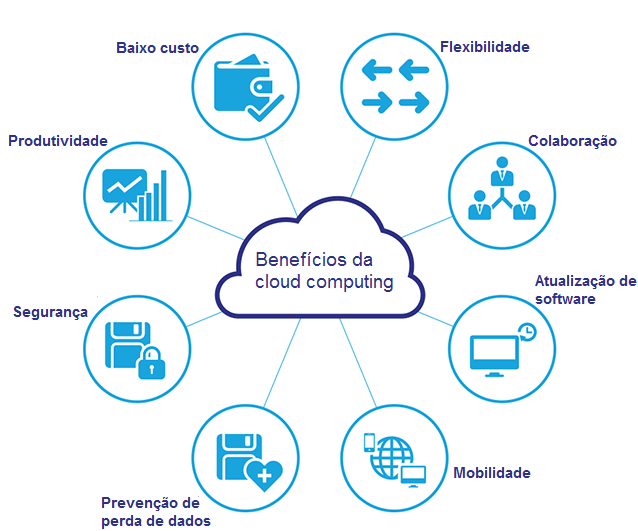
\includegraphics[width=\textwidth]{images/cloud.png}
    \end{column}
\end{columns}
\end{frame}

%% --------------------------------------------------------

\begin{frame}{Sistemas de informação distribuídos}

Úteis em ambientes de trabalho onde
\begin{itemize}
    \item Existe um grande número de sistemas de informação
    \item Interoperabilidade entre sistemas é ruim
\end{itemize}

\vspace{0.5cm}

Um sistema de informação distribuído é um middleware que facilita a troca de dados entre diversos sistemas de informação presentes em um mesmo ambiente

\vspace{0.5cm}

O middleware deve prover transações
\begin{columns}[T]
    \begin{column}{.35\textwidth}
        \begin{itemize}
            \item Atômicas
            \item Consistentes    
        \end{itemize}
    \end{column}
    \begin{column}{.49\textwidth}
        \begin{itemize}
            \item Isoladas
            \item Duráveis
        \end{itemize}    
    \end{column}
\end{columns}
\end{frame}

%% --------------------------------------------------------

\begin{frame}{Sistemas de informação distribuídos}

\centering 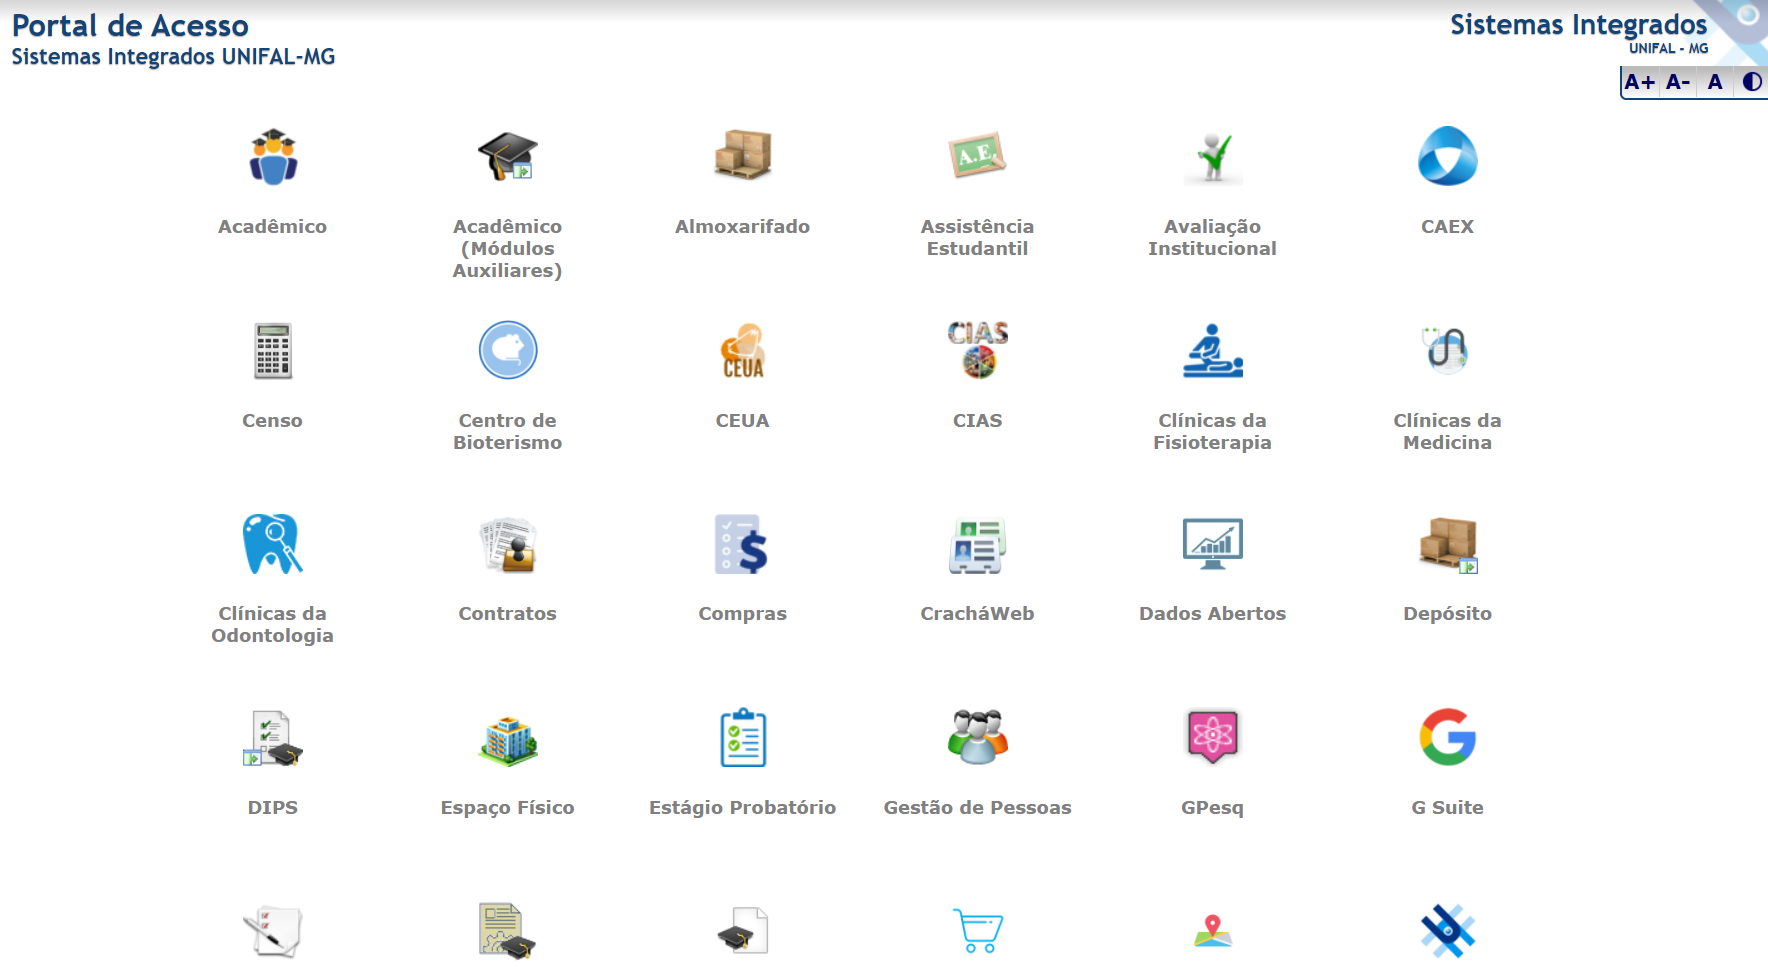
\includegraphics[width=\textwidth]{images/sistemas_unifal.png}

\end{frame}

%% --------------------------------------------------------

\begin{frame}{Sistemas pervasivos}

Sistemas ubíquos
\begin{itemize}
    \item Integrados naturalmente ao nosso ambiente
    \item Normalmente, não são percebidos pelas pessoas
\end{itemize}

\vspace{0.5cm}

São compostos por muitos
\begin{itemize}
    \item Sensores
    \item Atuadores
    \item Dispositivos móveis
\end{itemize}

\end{frame}

%% --------------------------------------------------------

\begin{frame}{Requisitos de sistemas pervasivos}

Distribuição
\begin{itemize}
    \item Nós são distribuidos pelo ambiente de forma transparente
\end{itemize}

\vspace{0.2cm}

Interação
\begin{itemize}
    \item A interação entre usuários e os nós é discreta
\end{itemize}

\vspace{0.2cm}

Sensíveis ao contexto
\begin{itemize}
    \item O sistema deve ser capaz de levar em consideração o contexto do usuário
\end{itemize}

\vspace{0.2cm}

Autonomia
\begin{itemize}
    \item O sistema deve ser capaz de operar sem interferência humana
\end{itemize}

\vspace{0.2cm}

Inteligência
\begin{itemize}
    \item Diversos tipos de ações e interações devem ser possíveis
\end{itemize}
\end{frame}

%% --------------------------------------------------------

\begin{frame}{Exemplo de sistema pervasivo}

\centering 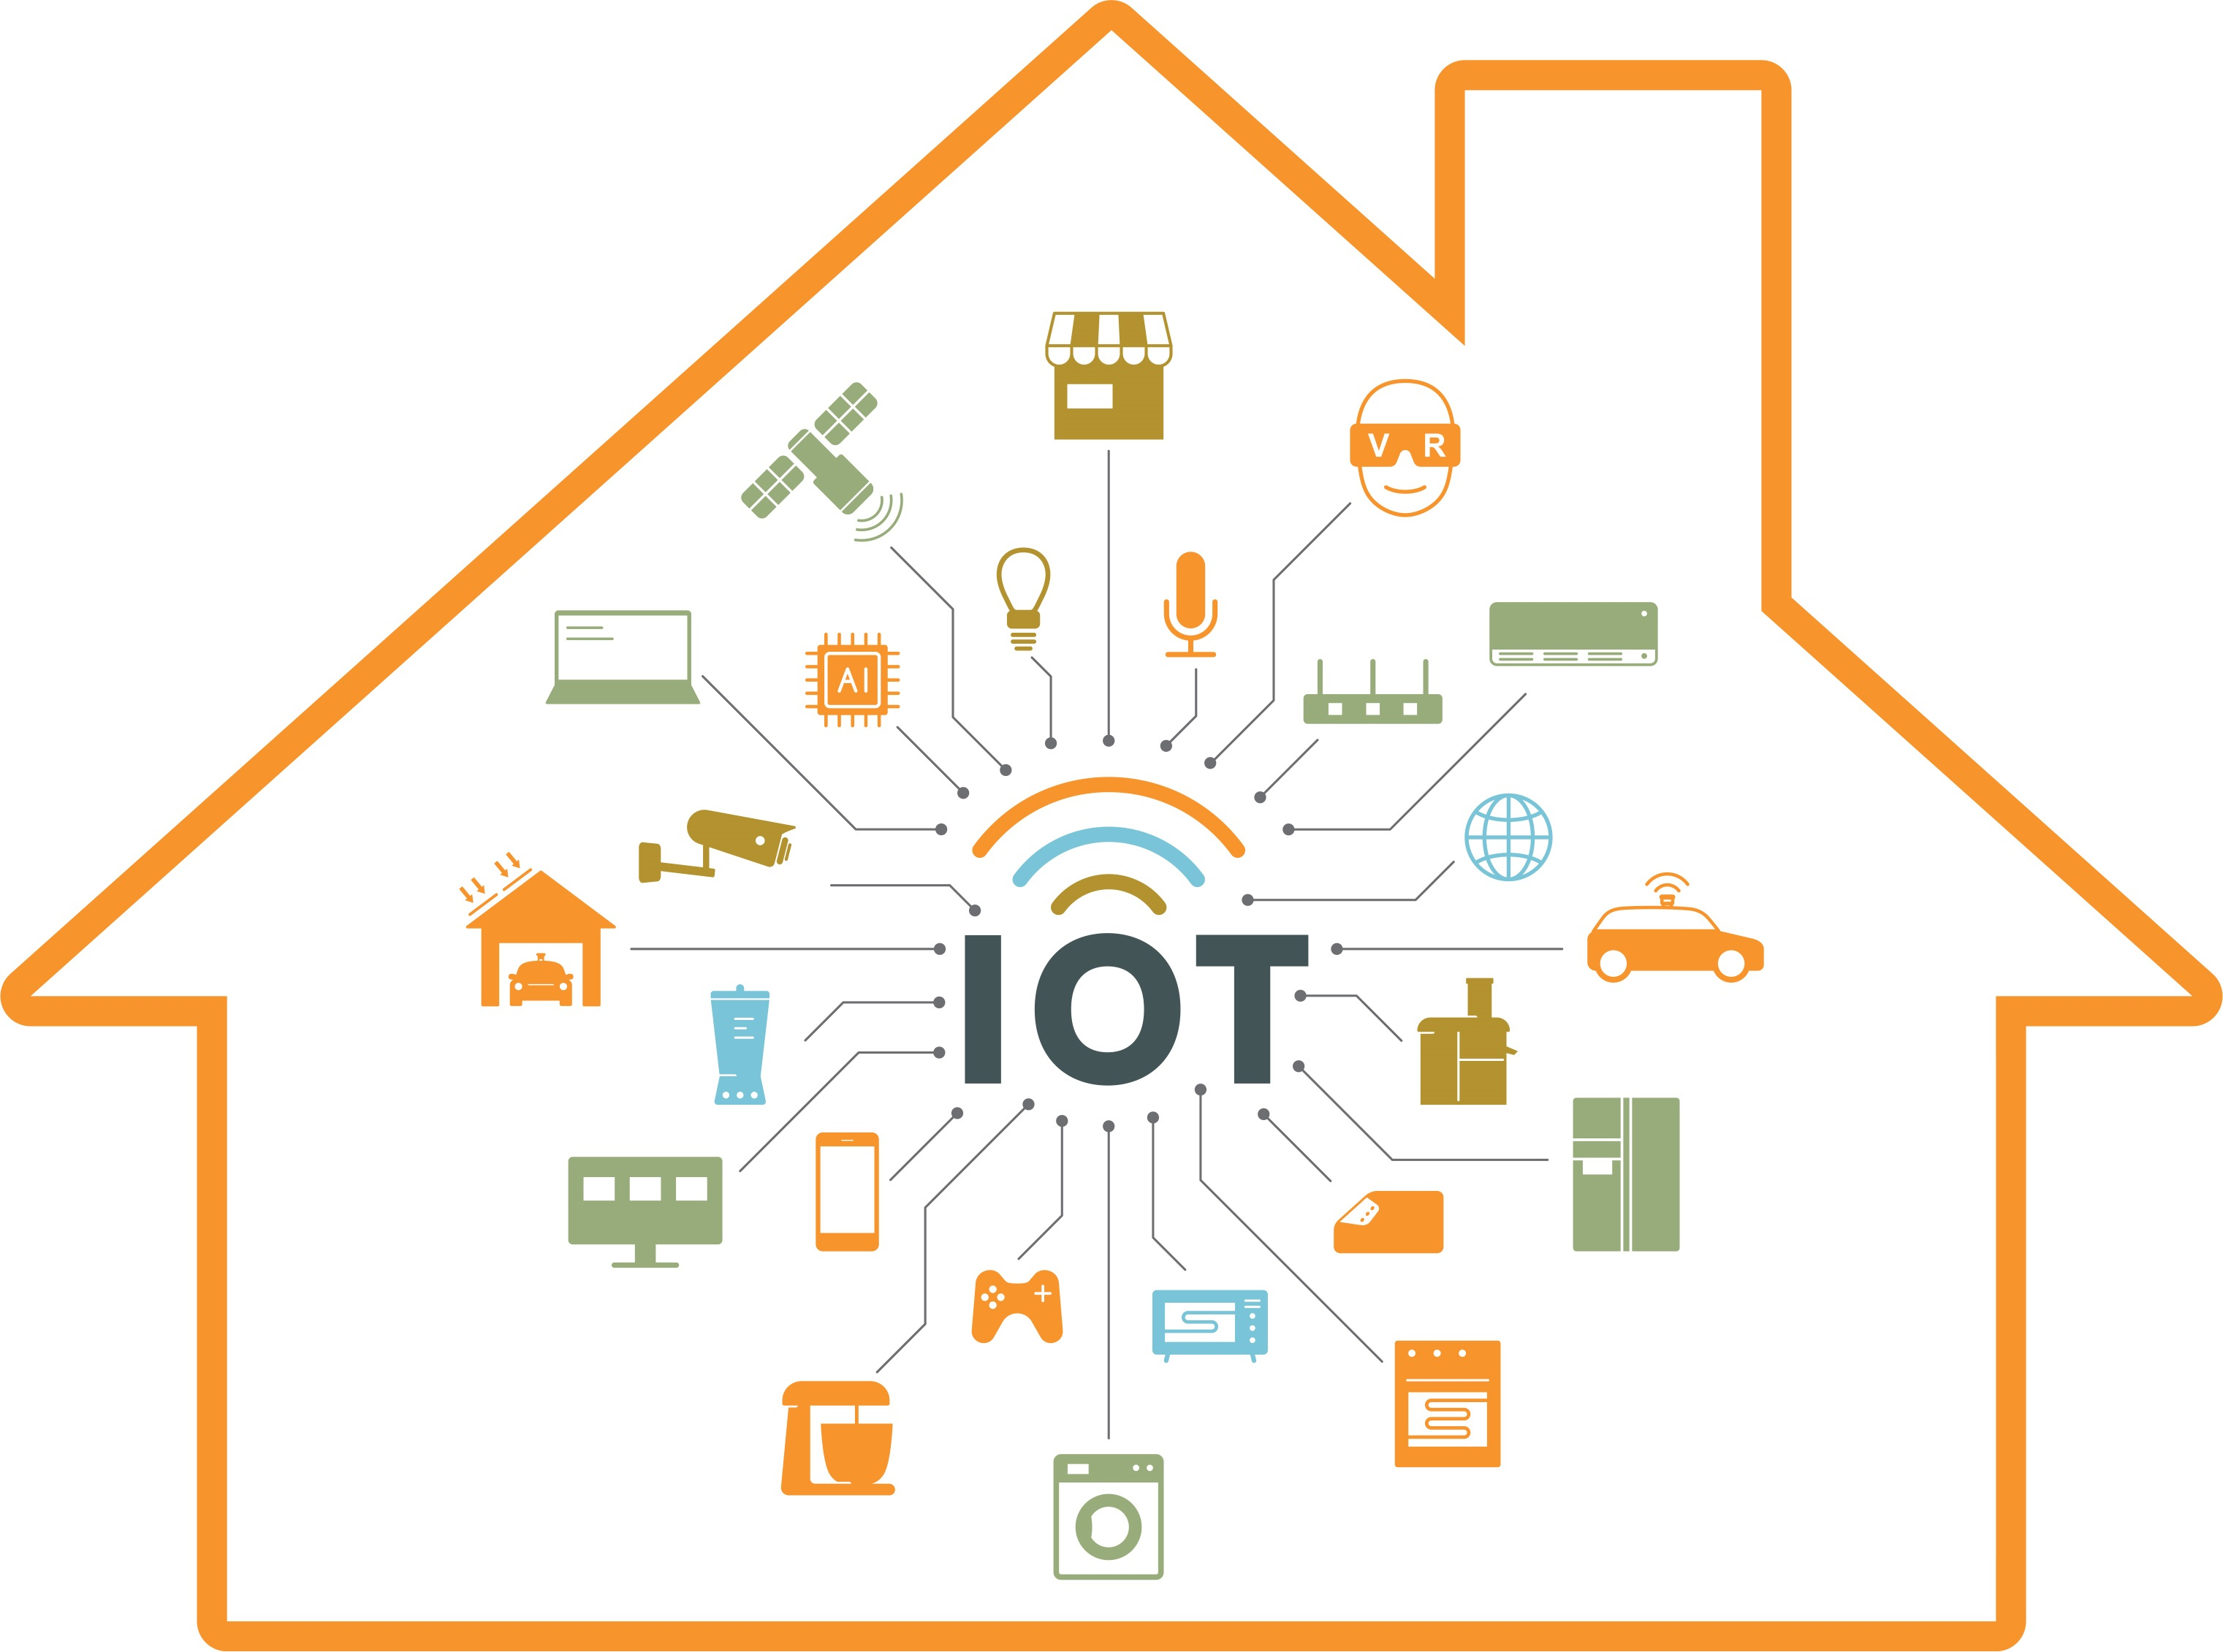
\includegraphics[width=\textwidth]{images/iot.jpg}

\end{frame}

\end{document}